\subsection{Error Pattern Assessment}
\label{sec:error_pattern_assessment}
\label{sec:error_pattern}

\begin{figure*}[htbp]
\centering
\subfigure[Single-Domain (vit-face)]{\label{fig:4a}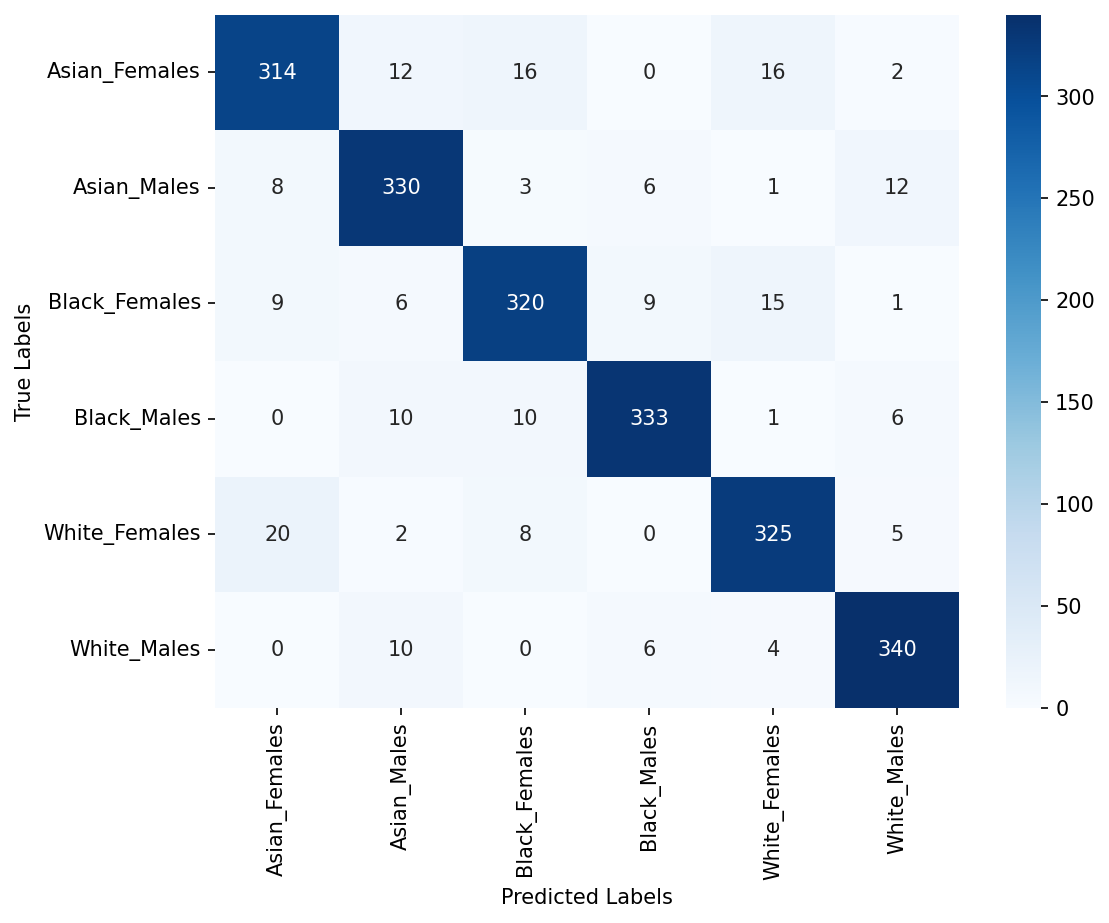
\includegraphics[width=0.32\textwidth]{images/confusion_matrix_single.png}}\hfill
\subfigure[Dual-Domain (vit-emotion-face)]{\label{fig:4b}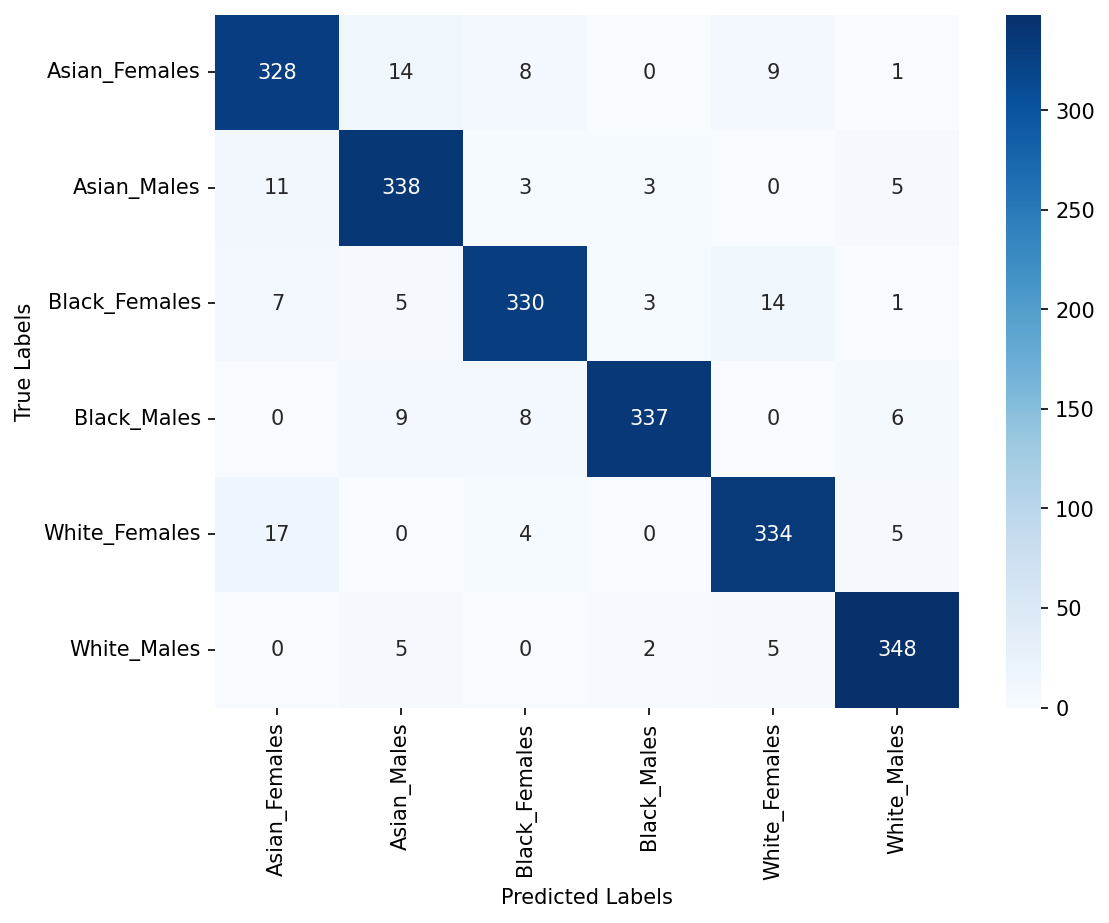
\includegraphics[width=0.32\textwidth]{images/confusion_matrix_dual.png}}\hfill
\subfigure[Tri-Domain (vit-face-emotion-age)]{\label{fig:4c}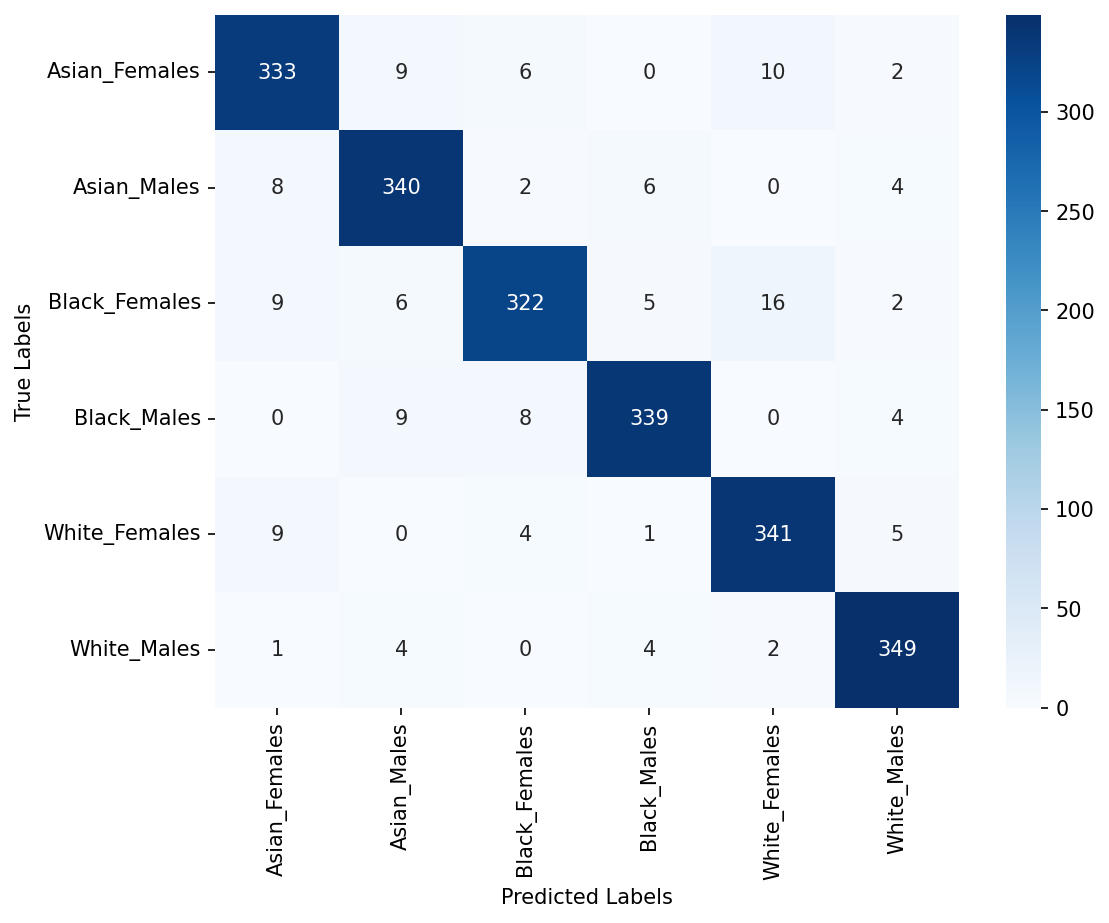
\includegraphics[width=0.32\textwidth]{images/confusion_matrix_svm_tri.png}}
\caption{Normalized Confusion Matrices of Selected Support Vector Machine Models on the Held-Out Test Set (N = 2,160): (a) Single-Domain (vit-face), (b) Dual-Domain (vit-emotion-face), and (c) Tri-Domain (vit-face-emotion-age).}
\label{fig:4}
\end{figure*}

The shift in classification error distributions from the single-domain scheme toward dual- and tri-domain configurations is analyzed through the confusion matrix diagrams in Figure~\ref{fig:4}, which encompass Figure~\ref{fig:4}(a), Figure~\ref{fig:4}(b), and Figure~\ref{fig:4}(c). Empirical evaluation reveals that the total misclassifications across the 2,160 held-out test data consistently decrease as the latent representation domains expand. The single-domain Face SVM model yields 198 prediction errors, which subsequently decrease to 145 samples in the dual-domain Emotion $\oplus$ Face scheme. The tri-domain Face $\oplus$ Emotion $\oplus$ Age configuration suppresses classification errors to the lowest point of 136 samples. This consistent reduction in errors indicates that multi-domain representation fusion sharpens the separation boundaries between demographic subgroups in the latent feature space.

An in-depth examination of the confusion matrix for the single-domain Face model in Figure~\ref{fig:4}(a) reveals that classification errors are predominantly concentrated in inter-racial subgroups within the same gender. This tendency is particularly pronounced in the female cohort, where the Asian Females subgroup incurs 46 misclassifications, encompassing 16 samples predicted as White Females and 16 samples as Black Females. Conversely, the White Females subgroup records 20 prediction errors distributed to Asian Females. This empirical pattern is consistent with the potential presence of inter-racial phenotypic overlap within single facial biometric geometric representations \cite{ref18}. Nevertheless, such confusion matrix evidence does not prove that visual overlap is the sole cause of all observed misclassifications.

The shift in classification error distributions in the dual-domain Emotion $\oplus$ Face model is further analyzed based on the confusion matrix in Figure~\ref{fig:4}(b). The addition of affective expression latent representations effectively reduces the inter-racial misclassifications among same-gender subgroups, particularly within the female group. Prediction errors from Asian Females to White Females are substantially suppressed from 16 cases to 9 cases. Concurrently, correctly predicted samples (true positives) in the White Females subgroup increase from 325 images to 334 images. Integrating dynamic facial expression signals strengthens inter-racial visual discriminant boundaries, enabling the classifier to distinguish similar morphological features with a more robust and stable certainty.

The misclassification patterns in the tri-domain Face $\oplus$ Emotion $\oplus$ Age configuration are comprehensively evaluated based on the confusion matrix in Figure~\ref{fig:4}(c). The integration of age-domain representations consistently increases the number of correct predictions in the Asian Females subgroup to 333 samples and White Females to 341 samples. Furthermore, cross-gender misclassifications, representing instances where female subjects are confused as male or vice versa, amount to only 51 cases out of the 2,160 held-out test data (2.36\%). These empirical findings indicate that inter-gender boundaries are separated very distinctly within the multi-domain latent representation space, such that the remaining classification errors in the tri-domain model are almost entirely dominated by inter-racial misclassifications within the same gender group.

